% !TeX program = xelatex
\documentclass[11pt,a4paper]{article}
\usepackage[margin=2.2cm]{geometry}
\usepackage{amsmath,amssymb,booktabs,tabularx,array,graphicx,enumitem,xcolor,hyperref,float}
\hypersetup{colorlinks=true,linkcolor=black,urlcolor=blue}
\setlength{\parskip}{0.45em}\setlength{\parindent}{0pt}
\setlength{\emergencystretch}{2em}
\renewcommand{\arraystretch}{1.2}
\setlist{nosep,leftmargin=1.6em}
\graphicspath{{../../Figures/v7_init_test/}}
\newcolumntype{L}{>{\raggedright\arraybackslash}X}
\newcolumntype{P}[1]{>{\raggedright\arraybackslash}p{#1}}
\title{Model 1 on the v7 data: Vegetation--Water--Sand Dynamics\\[2pt]\large Rebuilt version, 2026-11-10}
\author{2026 CQU\_MCM Problem B, Task 1}
\date{}
\begin{document}
\maketitle
\begin{quote}\small\bfseries
HISTORICAL DRAFT -- superseded by the 2026-11-10 audit. The old numbers and figures
below are not current results. Dynamic water storage was missing; pixel-level QA
has been corrected; free r, d and K are structurally non-identifiable; the selected
greening cohort is retrospective, not independent forecast validation.
Current equations: the correction in Reports/model\_v7.pdf.
Current numerical results: Results/v7/model1/.
\end{quote}


\noindent\textbf{What this is.} Model 1 rebuilt on the v7 data panel. It keeps the yearly state equation of \texttt{Reports/model\_v7.tex} unchanged, adds one water relation, and fits only the two parameters the data can identify. All numbers come from \texttt{Code/v7\_model1.py} and are stored in \texttt{Results/v7/model1/}. The detailed evidence is in \texttt{Docs/20261110\_model1\_v7\_rebuild.md}.

\section{The model}
\textbf{Vegetation} (v7 equation, yearly step; $V$ in \% cover, v7 units):
\begin{equation}
V_{t+1}=V_t+\underbrace{r\,V_t\Bigl(1-\frac{V_t}{K}\Bigr)W_t}_{\text{growth}}-\underbrace{d\,V_t}_{\text{decay}}-\underbrace{k\,E_t\Bigl(1-\eta\frac{V_t}{K}\Bigr)V_t}_{\text{wind erosion}} .
\end{equation}
\textbf{Effective soil moisture} (added relation):
\begin{equation}
W_t=\min\Bigl\{1,\ \frac{A_t}{c\,\min(1,2f_{c,t})\,\mathrm{ET}_{0g}}\Bigr\},\qquad
A_t=\eta_w I_t+G,\qquad f_{c,t}=\frac{V_t}{V_{\mathrm{full}}} .
\end{equation}
$W$ is the water plants can use divided by what the canopy would transpire without stress. $I$ is gross irrigation (mm/yr), $G$ groundwater supply, $\mathrm{ET}_{0g}=\sum_m f(T_m)\,\mathrm{ET}_{0,m}$ the temperature-weighted reference evapotranspiration, $f_c$ the ground-cover fraction. Root-zone storage (about 75 mm) is small against yearly fluxes of hundreds of mm, so at a yearly step moisture follows supply and demand and needs no storage equation.

\textbf{Couplings.} Water $\to$ vegetation: $W$ scales growth. Vegetation $\to$ water: more cover raises demand and lowers $W$. Vegetation $\to$ sand: the shelter factor $(1-\eta V/K)$. Sand $\to$ vegetation: the erosion term.

\textbf{Steady state.} For given $W$ the v7 closed form still holds:
\begin{equation}
x^*=\frac{V^*}{K}=\frac{rW-d-kE}{rW-kE\eta},\qquad\text{and with }W=1,\ k=0:\quad x^*=1-\frac{d}{r}=0.80 .
\end{equation}

\begin{table}[H]\small
\begin{tabularx}{\linewidth}{@{}P{2.2cm}P{5.2cm}L@{}}
\toprule
Parameter & Value & Status\\
\midrule
$r$ & $0.584\pm0.180$ yr$^{-1}$ & fitted, pooled over 7 stations\\
$d$ & $0.117\pm0.035$ yr$^{-1}$ & fitted, pooled over 7 stations\\
$K$ & $1.15\times Q_{0.95}$ of training-period $V$, per site; 38.1\% on the section & v7 rule, unchanged\\
$k$ & 0 (estimate $0.00\pm0.27$) & not identified; scenario range 0--0.10\\
$\eta$ & 1 & fixed; not identifiable\\
$c$ & 1.0 & assumption, range 0.7--1.2 (FAO-56)\\
$\eta_w$ & 0.75 & assumption, range 0.65--0.85\\
$V_{\mathrm{full}}$ & 66.6\% (v7 units) & from oasis pixels on the section\\
$\mathrm{ET}_{0g}$ & 1163 mm/yr & v7 panel, stations YT and MF\\
\bottomrule
\end{tabularx}
\end{table}

\section{Data}
\begin{table}[H]\small
\begin{tabularx}{\linewidth}{@{}P{4.3cm}P{5.2cm}L@{}}
\toprule
Data & Source & Used for\\
\midrule
v7 monthly panel, 9 stations, 2015--2025 & NASA POWER, MODIS MOD13Q1, ERA5 (\texttt{Data/v7/processed/}) & yearly $V$, $E$, ET$_0$; fitting $r$, $d$\\
217 pixels that went from bare sand to vegetation, 2003--2021 & MODIS MOD13Q1 on the Yutian--Minfeng margin (\texttt{Data/v7/section\_modis/}) & independent check of $r$, $d$\\
\bottomrule
\end{tabularx}
\end{table}
Yearly $V$ is the mean of observed June--September months. Seven stations are vegetated (YT, MF, QM, RQ, KEL, YL, ALE); XT and TZ are desert. Target years to 2022 are used for fitting, 2023--2025 are held out.

\section{What was checked in v7 and changed}
\begin{table}[H]\small
\begin{tabularx}{\linewidth}{@{}P{0.5cm}P{4.0cm}P{5.6cm}L@{}}
\toprule
 & Finding & Evidence & Change\\
\midrule
C1 & Fitting four parameters per station on 8 yearly points does not work & v7 ablation table: median training $R^2$ 0.004; 89\% of fits end on a bound & one parameter set shared by all vegetated stations, $K$ local\\
C2 & $k$ and $\eta$ cannot be estimated & adding $k$: AIC $-282.4\to-280.4$, $k=0.00\pm0.27$; adding $\eta$: condition number $2.6\times10^{8}$ & keep $(r,d)$; $k$, $\eta$ stay as scenario parameters\\
C3 & The v7 water index (normalised GWETROOT) has no time signal & 99.94\% of its variance is between stations; yearly s.d.\ within a station 0.003--0.013; no irrigation in the reanalysis & $W$ from the water relation; $W=1$ at irrigated oasis stations in the fit\\
C4 & $f(T)$ cannot be separated from $r$ at a yearly step & yearly mean temperature varies by at most 1.8\,$^\circ$C within a station & $f(T)$ absorbed in $r$; kept inside ET$_{0g}$\\
C5 & Imputed NDVI months were scored & 9.3\% of station-months imputed, 31\% at KEL & only observed months enter yearly $V$\\
C6 & Fixed end-members 0.05/0.85 understate ground cover & densest oasis pixels reach NDVI 0.583, i.e.\ 66.6\% in v7 units & divide by $V_{\mathrm{full}}$ where a ground fraction is needed\\
C7 & Task 2 used $K_s=0.45+0.55\,I/60$ without basis & \texttt{v7\_ablation.py} & replaced by the curve in Section 5\\
\bottomrule
\end{tabularx}
\end{table}

\section{Data support}
\begin{table}[H]\small\centering
\begin{tabular}{@{}lccc@{}}
\toprule
Stations, one year ahead ($V/K$) & Training RMSE & Hold-out RMSE & Hold-out $R^2$\\
\midrule
Model $(r,d)$ & 0.054 & 0.068 & 0.40\\
Persistence (next year = this year) & 0.060 & 0.058 & --\\
Station mean & -- & 0.079 & --\\
\bottomrule
\end{tabular}
\end{table}
The model beats the station mean but not persistence on the hold-out years. The station series sit near their steady state, so they fix the ratio $d/r$ and a relaxation rate, not much more.

\begin{table}[H]\small\centering
\begin{tabular}{@{}lcc@{}}
\toprule
Section pixels ($R^2$) & CON1--3 ($K$, $V_0$ fitted) & CON4 (never used)\\
\midrule
Station $r$, $d$ transferred, not refitted & 0.40 & 0.31\\
All four parameters fitted freely & 0.40 & 0.29\\
Mean baseline & 0.00 & $-0.02$\\
\bottomrule
\end{tabular}
\end{table}
A free fit to the pixels gives $r=0.64$, $d=0.10$, against $0.58$ and $0.12$ from the stations. Two data sets with different sites, years and dynamics agree; this is the main support for $r$ and $d$.

\begin{figure}[H]\centering
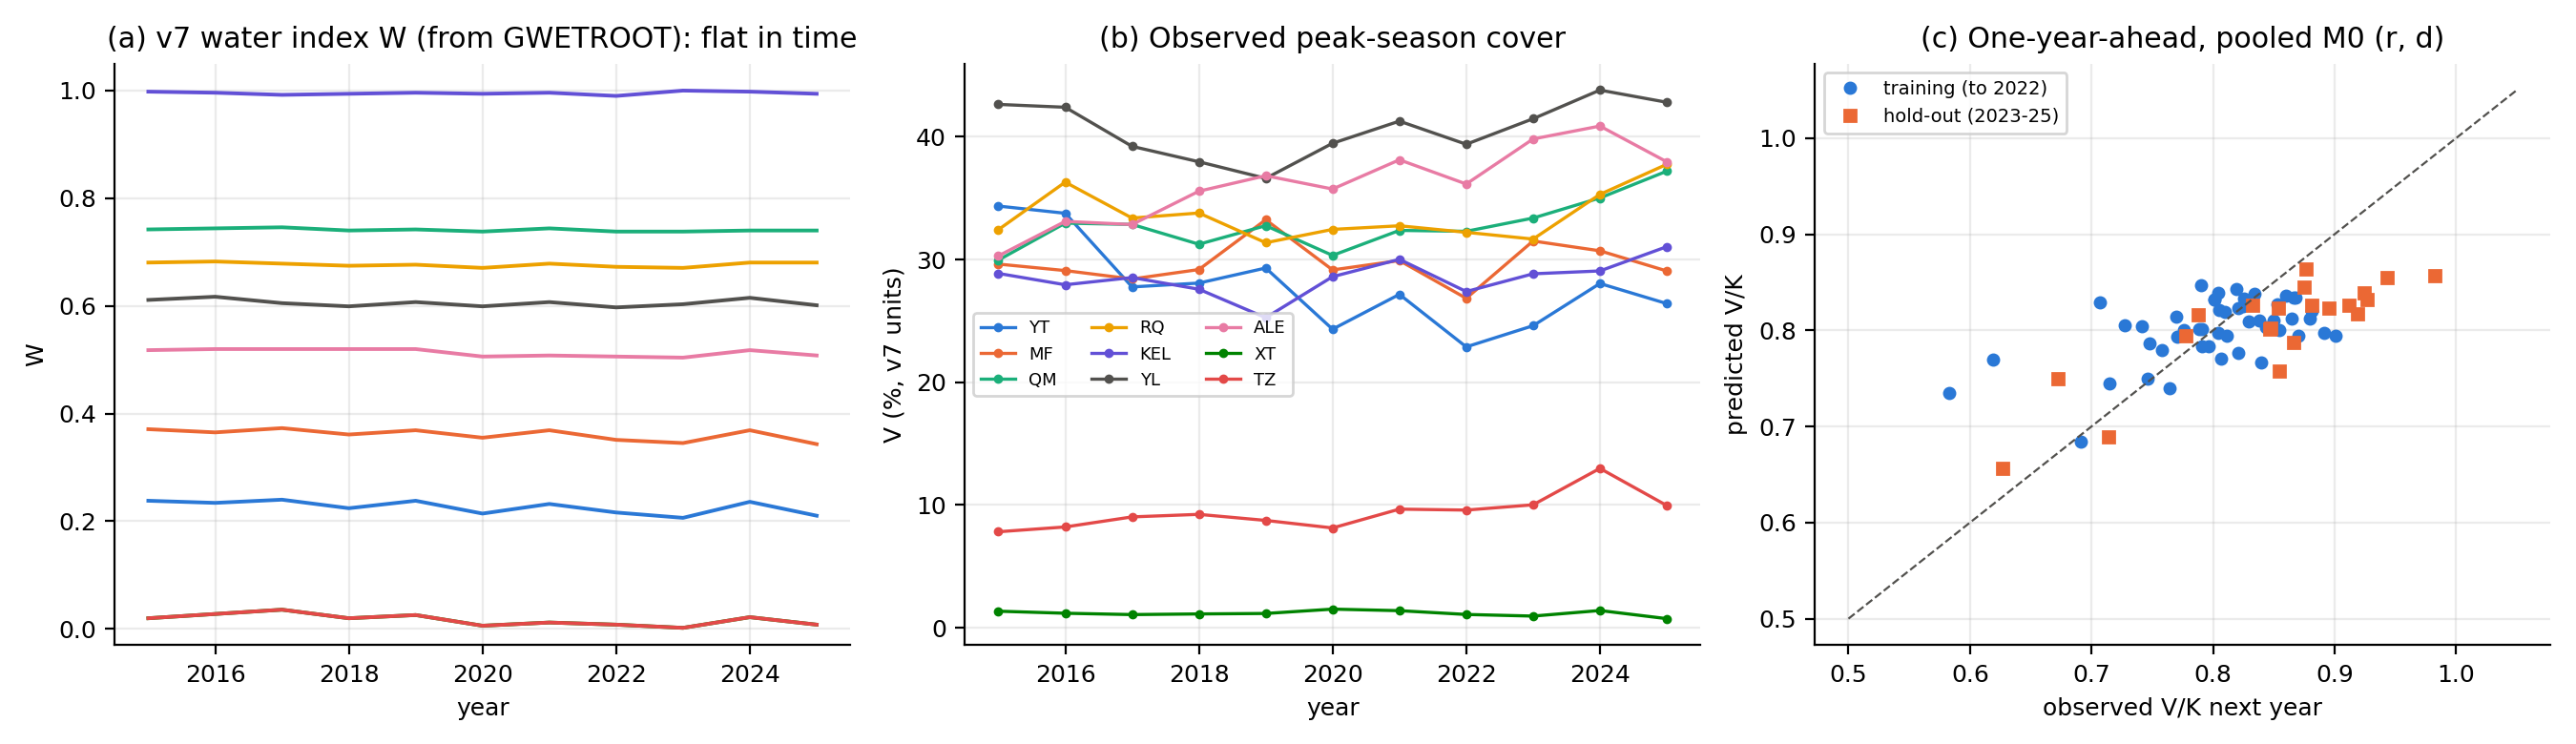
\includegraphics[width=\linewidth]{m1_fig1_station_evidence.png}
\caption{(a) The v7 water index is flat in time. (b) Observed peak-season cover. (c) One-year-ahead prediction of the pooled model.}
\end{figure}

\section{Results}
\begin{table}[H]\small\centering
\begin{tabular}{@{}lrrrrrrrr@{}}
\toprule
Gross irrigation (mm/yr) & 0 & 100 & 200 & 300 & 400 & 600 & 800 & 1000\\
\midrule
Steady $V$ (\%, v7 units) & 0 & 8.3 & 13.7 & 17.4 & 20.1 & 23.9 & 26.3 & 28.1\\
Ground-cover fraction & 0 & 0.13 & 0.21 & 0.26 & 0.30 & 0.36 & 0.40 & 0.42\\
$W$ & 0 & 0.26 & 0.31 & 0.37 & 0.43 & 0.54 & 0.65 & 0.77\\
Erosion relative to bare sand & 1.00 & 0.78 & 0.64 & 0.54 & 0.47 & 0.37 & 0.31 & 0.26\\
\bottomrule
\end{tabular}
\end{table}
\begin{itemize}
\item 1 mm/yr equals 10 m$^3$/ha/yr. Water stops limiting at about 1420 mm/yr.
\item A new planting reaches 90\% of its steady cover in 10--11 years.
\item Rain only: cover goes to zero (XT station 1.2\%; section desert pixels 0.2\%).
\item The natural ecotone (8.9\% in v7 units) corresponds to about 81 mm/yr of groundwater supply.
\item Steady cover at 300 mm/yr ranges from 14 to 21\% across the sensitivity cases; $r$, $d$ and $c$ matter most.
\end{itemize}
\begin{figure}[H]\centering
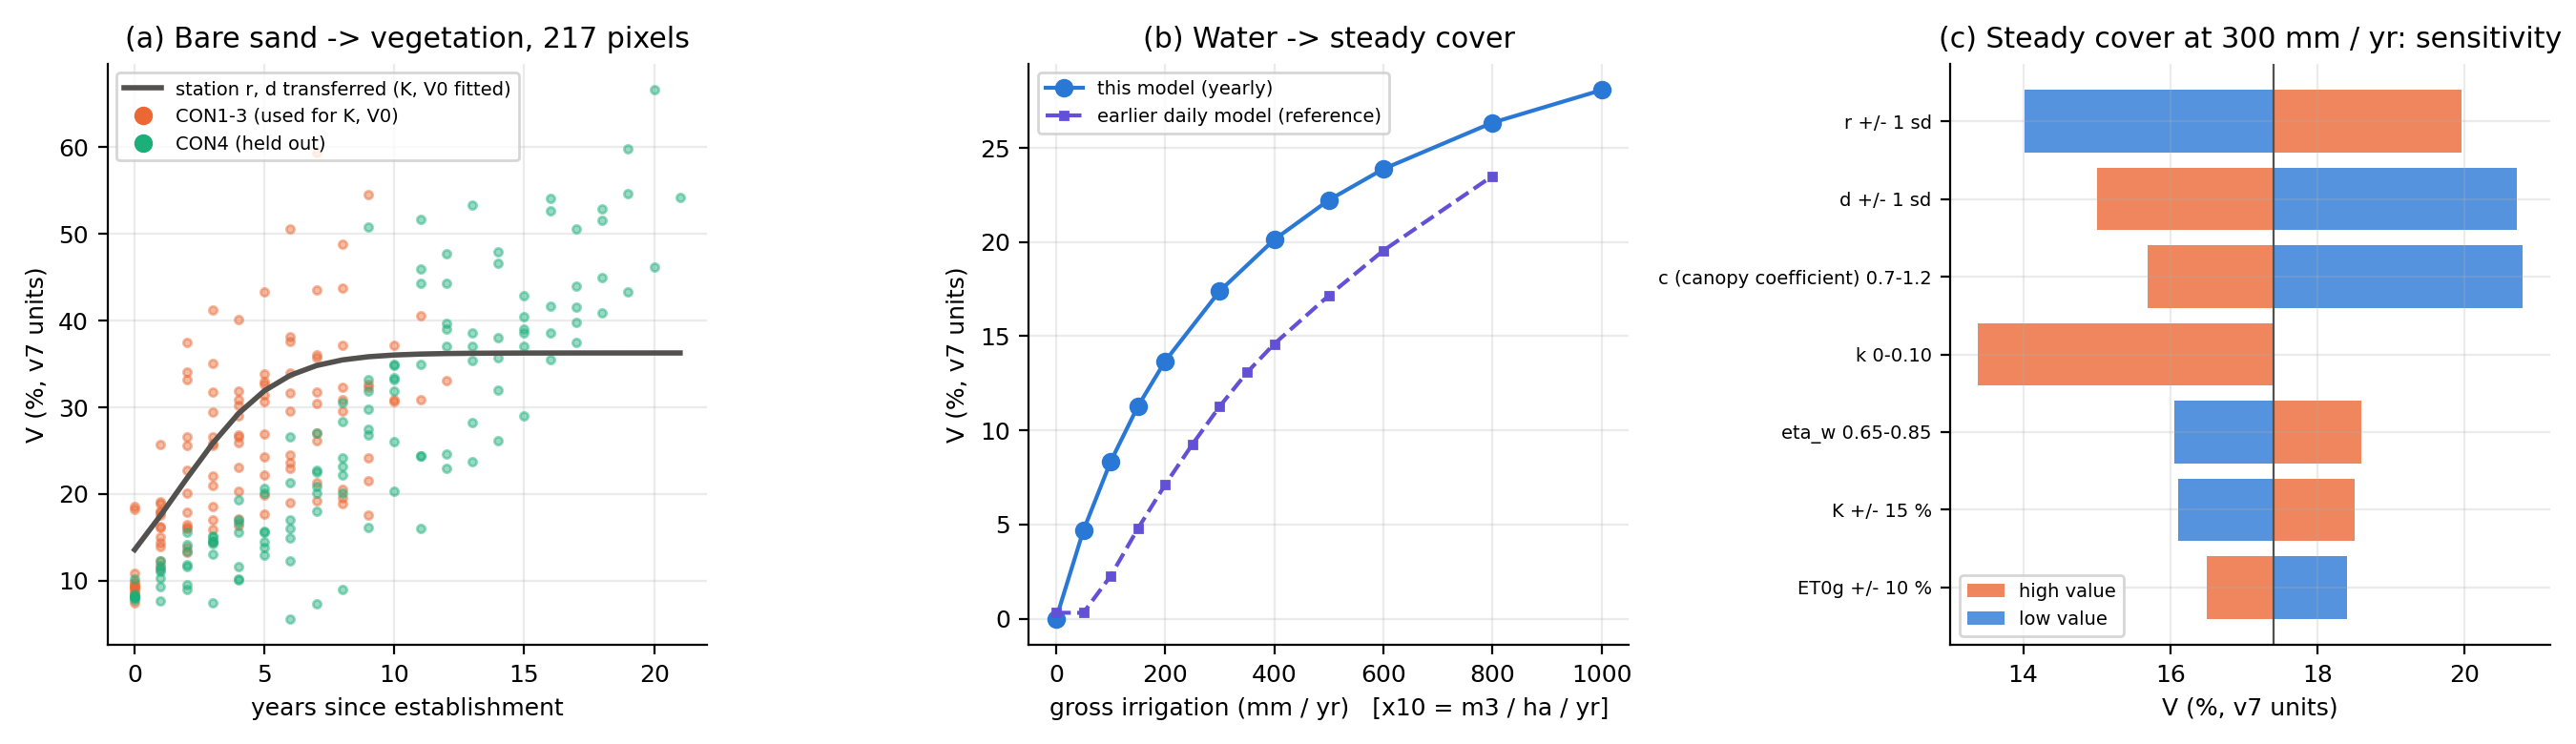
\includegraphics[width=\linewidth]{m1_fig2_transfer_and_water.png}
\caption{(a) Station parameters transferred to bare-to-vegetated pixels. (b) Water to steady cover, with the earlier daily model as reference. (c) Sensitivity of steady cover at 300 mm/yr.}
\end{figure}

\section{Limits}
\begin{enumerate}
\item One-year-ahead station cover is not predicted better than persistence.
\item The water-limited part of the curve has no measurement behind it; it depends on the assumed $c$ and $\eta_w$.
\item When irrigation stops the model loses cover at rate $d$ only (half-life 5.9 years). $d$ was measured on watered vegetation, so real loss is probably faster; Task 3 should treat this as a scenario.
\item $k$ is not identified; wind enters Task 3 as a scenario.
\item Stations are town coordinates inside oases and describe irrigated fringe vegetation, not shrub belts on dunes.
\end{enumerate}
\end{document}
